\chapter{Integrali curvilinei e potenziali}

In questo capitolo andremo a generalizzare il concetto di integrale di Riemann con il concetto di integrale curvilineo, il quale consente di valutare una funzione muovendosi lungo una qualunque direzione, e il concetto di potenziale, il quale ricopre una grandissima importanza in Fisica.

\section{Curve e integrali curvilinei}

Vogliamo estendere il concetto di integrale di Riemann: il primo passo è definire il concetto di \emph{integrale curvilineo}, ovvero l'integrale dove ci muoviamo lungo una \emph{direzione} data dalla curva $\gamma$. Per fare ciò, dobbiamo però richiedere un certo tipo di regolarità da questa curva per non avere problemi nell'integrazione.
\begin{definition}[curva $C^1$ a tratti]
	Sia $\gamma: [a, b] \to \mathbb{R}^n$. Diremo che $\gamma$ è $C^1$ a tratti se $\exists k \in \mathbb{N} : \exists t_0, \ldots, t_k \in [a, b], a = t_0 < \ldots < t_k = b$ tali che $\gamma \in C^1([t_{j}, t_{j+1}]) \, \forall j \in \{0, \ldots, k-1 \}$ e $\gamma \in C^0([a, b])$.
\end{definition}
Possiamo anche definire la famiglia di curve $C^1$ a tratti su $[a,b]$
\begin{definition}[famiglie delle curve $C^1$ a tratti]
	Indichiamo con $C^1_{\text{tratti}}([a, b], \mathbb{R}^n)$ la famiglia di tutte le curve a tratti su $[a, b]$
\end{definition}
Se vogliamo specificare la suddivisione $a=t_0 < t_1 < \ldots < t_k = b$ per la quale la curva $\gamma \in C^1([t_j, t_{j+1}], \mathbb{R}^n) \, \forall j \in \{1, \ldots, k \}$ 
diremo che la curva $\gamma$ è $C^1$ a tratti rispetto alla suddivisione (o partizione) $a = t_0 < \ldots < t_k = b$. \\
\begin{definition}[lunghezza di una curva $\gamma$] 
	Sia $\gamma : [a,b] \to \mathbb{R}^n$, definiamo la lunghezza di $\gamma$ come
	$$
		\mathit{l}(\gamma) = \sup \left\{ \sum_{j=1}^k |\gamma(t_j)-\gamma(t_{j-1})| : a = t_0 < t_1 < \ldots < t_k = b, \, k \in \mathbb{N}^+ \right\}
	$$
\end{definition}
Consideriamo adesso una curva $\gamma \in C^1_{\text{tratti}}([a, b], \mathbb{R}^n)$ rispetto alla suddivisione $a=t_0 < t_1 < \ldots < t_k = b$ allora definiamo
$$
\int_a^b |\dot{\gamma}(t)|dt = \sum_{j=1}^k \int_{t_{j-1}}^{t_j} |\dot{\gamma}(t)|dt 
$$
e possiamo verificare che l'integrale non dipende dalla suddivisione rispetto la quale $\gamma$ è $C^1$ a tratti, infatti se esistesse un'altra suddivisione $a=\tau_0 < \tau_1 < \ldots < \tau_p = b$ allora
$$
\sum_{i=1}^k \int_{t_{i-1}}^{t_{i}} |\dot{\gamma}(t)|dt = \sum_{i=1}^p \int_{\tau_{i-1}}^{\tau_{i}} |\dot{\gamma}(t)|dt
$$
\begin{theorem}
Se $\gamma \in C^1_{\text{tratti}}([a, b], \mathbb{R}^n)$ allora
$$
\mathit{l}(\gamma) = \int_a^b |\dot{\gamma(t)}|
$$
\end{theorem}
\begin{proof}
Possiamo innanzitutto osservare che, fissando una parametrizzazione $a=t_0 < t_1 < \ldots < t_k = b$ per cui la curva $\gamma \in C^1_\text{tratti}([a, b])$, allora:
$$
	\sum_{j=1}^k |\gamma(t_j) - \gamma(t_{j-1})| = \sum_{i=1}^k |\int_{t_{j-1}}^{t_j} \dot{\gamma}(t)dt| \leq \sum_{i=1}^k \int_{t_{j-1}}^{t_j} |\dot{\gamma}(t)dt| = \int_a^b |\dot{\gamma}(t)dt|
$$
dunque, siccome la parametrizzazione scelta è arbitraria, allora
$$
l(\gamma) = \sup \left\{ \sum_{j=1}^k |\gamma(t_j) - \gamma(t_{j-1})| : a = t_0 < t_1 < \ldots < t_k = b, \, k \in \mathbb{N}^+ \right\} \leq \int_a^b |\dot{\gamma}(t)|dt
$$
Possiamo, per concludere la dimostrazione, osservare che $\dot{\gamma}$, per il teorema di Heine-Cantor, è uniformemente continua (siccome $\gamma \in C_\text{tratti}^1$, la sua derivata sarà continua $\forall x \in (t_{i-1}, t_i) \, \, \forall i$), ovvero
$$
\forall \varepsilon > 0, \exists \delta > 0: \forall x, y, |x-y| < \delta \implies |\dot{\gamma}(x) - \dot{\gamma}(y)| < \varepsilon
$$
e possiamo allora prendere una suddivisione tale che $\max\{t_{j+1} - t_{j}\} < \delta$ in maniera tale che
$$
|\gamma(x)-\gamma(y)| \leq \varepsilon \, \, \forall x, y \in [t_j, t_{j+1}]
$$
dunque
$$
\gamma(t_{j+1}) - \gamma(t_j) = \int_{t_j}^{t_{j+1}} \dot{\gamma}(t)dt = \int_{t_j}^{t_{j+1}} (\dot{\gamma}(t) - \dot{\gamma}(s) + \dot{\gamma}(s)dt) = \int_{t_j}^{t_{j+1}} (\dot{\gamma}(t) - \dot{\gamma}(s))dt + \dot{\gamma}(s)(t_{j+1} - t_j).
$$
Esplicitiamo a questo punto il termine con $\dot{\gamma}(s)$ e passiamo ai valori assoluti:
\begin{align*}
&|\dot{\gamma}(s)|(t_{j+1} - t_j) \leq |\gamma(t_{j+1}) - \gamma(t_j) - \int_{t_j}^{t_{j+1}} (\dot{\gamma}(t) - \dot{\gamma}(s))dt| \stackrel{\text{dis. triang}}{\leq} \\
&\stackrel{\text{dis. triang}}{\leq} |\gamma(t_{j+1}) - \gamma(t_j)| + |\int_{t_j}^{t_{j+1}} (\dot{\gamma}(t) - \dot{\gamma}(s))dt| \stackrel{|\dot{\gamma}(t)-\dot{\gamma}(s)| \leq \varepsilon}{\leq} |\dot{\gamma}(t_{j+1}) - \dot{\gamma}(t_j)| + \varepsilon(t_{j+1} - t_{j})
\end{align*}
dividendo per $t_{j+1} - t_j$ concludiamo che
$$
|\dot{\gamma}(s)| \leq \frac{|\gamma(t_{j+1})-\gamma(t_j)|}{t_{j+1} - t_j} + \varepsilon
$$
e, integrando per $s \in [t_j, t_{j+1}]$, avremo che
$$
\int_{t_{j}}^{t_j} |\dot{\gamma}(s)|ds \leq \int_{t_j}^{t_{j+1}} \frac{|\gamma(t_{j+1} - \gamma(t_j)|)}{t_{j+1}-t_j} ds + \int_{t_j}^{t_{j+1}} \varepsilon ds = |\gamma(t_{j+1})-\gamma(t_j)| + \varepsilon(t_{j+1} - t_j)
$$
sommando adesso sulle $j$ avremo che
$$
\int_a^b |\dot{\gamma}(s)|ds \leq \sum_{j=1} |\gamma(t_{j+1})-\gamma(t_j)| + \varepsilon(b-a) \leq l(y) + \varepsilon(b-a) 
$$
ma, siccome $\varepsilon$ è arbitrario, per $\varepsilon \to 0$ ricaviamo che
$$
\int_a^b |\dot{\gamma}(s)|ds \leq l(\gamma)
$$
ma allora segue necessariamente che $l(\gamma) = \int\limits_a^b |\dot{\gamma}(t)|dt$.
\end{proof}
\begin{remark}
Il risultato ottenuto è vero anche per curve lipschtziane, tuttavia va modificata leggermente la dimostrazione.
\end{remark}
\begin{remark}
$l(\gamma)$ misura quello che noi consideriamo come \emph{lunghezza} della curva solo se $\gamma$ è iniettiva, altrimenti misura la lunghezza dell'immagine della curva "con molteplicità".
\end{remark}
\begin{definition}
	Sia $\gamma \in C^1_{\text{tratti}}([a,b], \mathbb{R}^n)$ e $f: \gamma([a,b]) \to \mathbb{R}$ continua, definiamo l'integrale di lunghezza o l'integrale curvilineo di prima specie di $f$ lungo $\gamma$ come
	$$
		\int_{\gamma} f = \int_a^b f(\gamma(t))|\dot{\gamma}(t)|dt
	$$
\end{definition}
%\begin{tikzpicture}
    % Axes
%    \draw[->] (-0.5, 0, 0) -- (6, 0, 0) node[right] {$x$};
%    \draw[->] (0, -0.5, 0) -- (0, 6, 0) node[above] {$y$};
%    \draw[->] (0, 0, -0.5) -- (0, 0, 5) node[above] {$z$};

    % Surface representing f(x, y)
%    \foreach \x in {0, 0.5, ..., 5} {
%        \foreach \y in {0, 0.5, ..., 5} {
%            \pgfmathsetmacro{\z}{0.1*\x^2 + 0.1*\y^2}
%            \fill[red!10] (\x, \y, 0) -- (\x, \y, \z) -- (\x+0.5, \y, \z) -- (\x+0.5, \y, 0) -- cycle;
%        }
%    }

    % Curve gamma
%    \draw[thick, blue, domain=0:5, smooth, variable=\t] plot ({\t}, {2*sin(\t r)}, {0.1*\t^3 - \t + 1}) node[right] {$\gamma$};

    % Area under the curve f \circ gamma
    %\fill[opacity=0.3, blue!30] plot[domain=0:5, smooth, variable=\t] ({\t}, {2*sin(\t r)}, 0) -- plot[domain=0:5, smooth, variable=\t] ({\t}, {2*sin(\t r)}, {0.1*\t^3 - \t + 1}) -- cycle;

    % Points on gamma
    %\fill[black] (1, {2*sin(1)}, {0.1*1^3 - 1 + 1}) circle (1.5pt) node[below left] {$\gamma(t_1)$};
    %\fill[black] (4, {2*sin(4)}, {0.1*4^3 - 4 + 1}) circle (1.5pt) node[below right] {$\gamma(t_2)$};

    % Indicating the integral
%    \node at (2.5, 2, 4) {$\int_{\gamma} f(x, y, z)\, \mathrm{d}s$};
%\end{tikzpicture}
\begin{theorem}
	Sia $\gamma \in C^1_{\text{tratti}}([a, b], \mathbb{R}^n)$ e $f \in C^1(\gamma([a, b]))$. Allora 
	$$
		\varphi: [c, d] \to [a, b]
	$$
	di classe $C^1$ e bigettiva. Allora $\gamma \circ \varphi \in C^1_{\text{tratti}}([c,d], \mathbb{R}^n)$ e
	$$
		\int_{\gamma} f = \int_{\gamma \circ \varphi} f
	$$
\end{theorem}
\begin{proof}
Siccome $\varphi: [c,d] \to [a,b]$ è bigettiva, allora dev'essere monotona. Facciamo la dimostrazione, senza perdita di generalità, nel caso in cui $\varphi$ è strettamente crescente
e possiamo definire $\tau_i = \varphi^{-1}(t_j)$ (che sarà strettamente crescente a sua volta grazie alla continuità della funzione $\varphi$), dunque
$$
\gamma \circ \varphi \in C^1([\tau_i, \tau_{i+1}], \mathbb{R}^n)
$$
(nel caso di $\varphi$ decrescente allora avevamo che $\gamma \circ \varphi \in C^1([\tau_{i+1}, \tau_{i}], \mathbb{R}^n)$) e la composizione di due funzioni continue è ancora una funzione continua, dunque
$\gamma \circ \varphi \in C^{0}([c, d], \mathbb{R}^n)$ e questo ci porta a concludere che
$$
\gamma \circ \varphi \in C^1_{\text{tratti}}([c, d], \mathbb{R}^n)
$$
Mostriamo adesso la tesi per i singoli intervalli nel caso in cui $\varphi$ è strettamente crescente
$$
\int_{t_i}^{t_{i+1}} f(\gamma(t))|\dot{\gamma}(t)|dt \stackrel{t = \varphi(\tau)}{=} \int_{\varphi^{-1}(t_{i})}^{\varphi^{-1}(t_{i+1})} f((\gamma \circ \varphi)(\tau))|\dot{\gamma}(\varphi(\tau))|\dot{\varphi}(\tau) d\tau
$$
\noindent e osserviamo che, siccome $\varphi$ è strettamente crescente, allora $\dot{\varphi}(\tau) = |\dot{\varphi}(\tau)|$, dunque (con un leggero abuso di notazione nelle variabili di integrazioni e sugli estremi di integrazione)
$$
\int_{\tau_i}^{\tau_{i+1}} f((\gamma \circ \varphi)(\tau))|\dot{\gamma}(\varphi(\tau))| \, |\dot{\varphi}(\tau)| d\tau = \int_{\tau_i}^{\tau_{i+1}} f( (\gamma \circ \varphi)(\tau) ) |\gamma \circ \varphi|'(\tau) d\tau.
$$
Sommando in $j$ otteniamo che
$$
\int_\gamma f = \sum_{i=1}^k \int_{t_i}^{t_{i+1}} f(\gamma(t))|\dot{\gamma}(t)|dt = \sum_{i=1}^l \int_{\tau_i}^{\tau_{i+1}} f((\gamma \circ \varphi)(\tau)) |\gamma \circ \varphi|'(\tau) d\tau = \int_{\gamma \circ \varphi} f 
$$
ovvero la tesi.
\end{proof}
\begin{cor}[lunghezza di un arco]
	Sia $f(x): I \to \mathbb{R}$ con $f \in C^1(I)$ allora la lunghezza dell'arco descritto da $f(x)$ è dato da
	$$
		\int_I \sqrt{1 + f'(x)}dx
	$$
\end{cor}
\begin{proof}
Dal teorema precedente, possiamo considerare la curva $\gamma: I \to \mathbb{R}^2$ tale che $\gamma = (t, f(t)) \, \forall t \in I$ e calcolare la lunghezza della curva con il teorema precedente:
$$
	\mathit{l}(\gamma) = \int_{I} |\dot{\gamma}(t)|dt = \int_I \sqrt{1 + (f'(t))^2} dt
$$
ovvero la tesi.
\end{proof}
\section{Integrali curvilinei su forme differenziali e campi vettoriali}

Abbiamo generalizzato l'integrale di Riemann all'integrale curvilineo come l'integrale di una funzione a valori reali lungo una direzione impartita dalla curva $\gamma$, vogliamo adesso generalizzarlo a funzioni a valori vettoriali. I candidati ideali per fare questo sono le forme differenziali e i campi vettoriali di cui richiediamo una certa regolarità
\begin{definition}[$1$-forma differenziale di classe $C^k$]
Sia $\Omega \subseteq \mathbb{R}^n$ un insieme aperto, allora $$\omega(x) = \sum_{j=1}^n a_j(x)dx_j$$ è una $1$-forma differenziale di classe
$C^k(\Omega)$, ovvero
$$
\omega \in C^k(\Omega, (\mathbb{R}^n)^*) \iff a_j \in C^k(\Omega) \, \forall j \in \{1, \ldots n \}
$$
\end{definition}
Diamo adesso la nozione di \emph{esattezza} di una forma differenziale
\begin{definition}[esattezza di una $1$-forma differenziale]
	Diremo che $\omega$ è esatta se esiste una primitiva $V \in C^1(\Omega)$ tale che
	$$
		dV = \omega
	$$
	ovvero se $\omega = \sum\limits_{j}^n a_j dx_j$ allora $a_j = \frac{\partial V}{\partial x_j}$ su $\Omega \, \forall j \in \{1, \ldots, n\}$
\end{definition}
Equivalentemente diamo la nozione di \emph{chiusura} di una forma differenziale
\begin{definition}
	Sia $\omega = \sum_{j=1}^n a_j dx_j \in C^k(\Omega, (\mathbb{R}^n)^*)$, ovvero una $1$-forma differenziale di classe $C^k(\Omega)$, allora diremo che
	è chiusa se abbiamo che
	$$
		\frac{\partial a_j}{\partial x_i} - \frac{\partial a_i}{\partial x_j} = 0 \, \forall i, j: 1 \leq i < j \leq n
	$$
\end{definition}
Equivalentemente, possiamo dare delle definizioni che sono "duali" nel caso, però, di campi vettoriali:
\begin{definition}[campo vettoriale di classe $C^k$]
	Sia $\Omega \subseteq \mathbb{R}^n$ un insieme aperto, allora $$F(x)=\sum_{j=1}^n f_j(x)e_j$$ è un campo vettoriale di classe $C^k$, ovvero 
	$$F \in C^k(\Omega, \mathbb{R}^n) \iff f_j \in C^k(\Omega) \, \forall j \in \{1, \ldots, n\} $$
\end{definition}
Nel caso di campi vettoriali la nozione di \emph{esattezza} e di \emph{chiusura} è sostituita dal concetto di \emph{campo conservativo} (che è un concetto che ogni fisico ha incontrato nel corso di Fisica 1
nel caso del moto in campo centrale per esempio) e dal concetto di \emph{campo irrotazionale}
\begin{definition}[campo conservativo]
	Diremo che $F$ è un campo conservativo se esiste un potenziale $V \in C^1(\Omega)$ tale che
	$$
	F = \nabla V
	$$
	ovvero se $F=(f_1, \ldots, f_n)$ e abbiamo che $f_j = \frac{\partial V}{\partial x_j}$ su $\Omega \, \forall j \in \{1, \ldots, n \}$
\end{definition}
\begin{definition}[campo irrotazionale]
	Sia  $\Omega \subseteq \mathbb{R}^n$ aperto e sia $F = \sum_{i=1}^n f_i e_i \in C^k(\Omega, \mathbb{R}^n)$ un campo vettoriale, diremo che $F$ è un campo irrotazionale se
	$$
	\frac{\partial f_i}{\partial x_j} - \frac{\partial f_j}{\partial x_i} = 0 \, \forall i, j: 1 \leq i < j \leq n
	$$
\end{definition}

Possiamo andare a definire il concetto di integrale curvilineo di seconda specie di $\omega$ (oppure di $F$) lungo una curva $\gamma$ come segue
\begin{definition}[integrale curvilineo di seconda specie di $\omega$ lungo una curva $\gamma$]
	Sia $\Omega \subseteq \mathbb{R}^n$, $\omega \in C^0(\Omega, (\mathbb{R}^n)^*)$ una $1$-forma differenziale e sia $\gamma \in C^1_{\text{tratti}}([a,b], \Omega)$ una curva. Definiamo l'integrale curvilineo di seconda specie di 
	$\omega$ lungo una curva $\gamma$ come
	$$
		\int_\gamma \omega = \sum_{i=1}^k \int_{t_{j-1}}^{t_j} \omega(\gamma(t))(\dot{\gamma}(t))dt
	$$
\end{definition}
\begin{definition}[integrale curvilineo di seconda specie di $F$ lungo una curva $\gamma$]
	Sia $\Omega \subseteq \mathbb{R}^n$, $F \in C^0(\Omega, \mathbb{R}^n)$ un campo vettoriale e sia $\gamma \in C^1_{\text{tratti}}([a, b], \Omega)$ una curva. Definiamo l'integrale curvilineo di seconda specie di 
	$F$ lungo una curva $\gamma$ come 
	$$
		\int_\gamma F = \sum_{i=1}^k \int_{t_{j-1}}^{t_j} \innerprod{F(\gamma(t))}{\dot{\gamma}(t)}dt
	$$
\end{definition}
\begin{remark}
Dalla definizione di una forma differenziale sappiamo che
$$
\omega(\gamma(t))(\dot{\gamma}(t)) = \sum_{i=1}^n a_i(\gamma(t))dx_i(\gamma(t)) = \sum_{i=1}^n a_i(\gamma(t))\gamma_i(t) 
$$
\end{remark}

\begin{remark}
Questa \emph{dualità} presente fra i campi vettoriali e le $1-$forme differenziali deriva dal fatto che, di fatto, questi sono la stessa cosa: infatti,
noi potremmo pensare di considerare $F \in C^0(\Omega, \mathbb{R}^n), F=(f_1, \ldots, f_n)$ e costruire una $1-$forma del tipo $\omega_F=f_1 dx_1 + f_2 dx_2 + \ldots + f_ndx_n$ come $1-$forma differenziale associata ad $F$ e osservare
che $\forall \gamma \in C^1_\text{tratti}([a, b], \Omega)$ abbiamo che
$$
\int_\gamma F = \int_\gamma \omega_F
$$
Viceversa, presa $\omega = \sum\limits_{i=1}^n a_i dx_i$ se definiamo $F_\omega = (a_1, a_2, \ldots, a_n) \implies$
$$
\int_\gamma \omega = \int_\gamma F_\omega
$$
Tali eguaglianze seguono immediatamente dalle definizioni e giustificano questa doppia formulazione che abbiamo dato. \\
Osservando la questione da un punto di vista più elevato, in presenza di metrica riemanniana, l'applicazione dell'operazione di contrazione fornisce un modo per far corrispondeere ad ogni campo vettoriale
una $1-$forma differenziale \emph{contraendo} il campo vettoriale con la metrica. Quindi da questo breve accenno senza formule, possiamo intuire che campi vettoriali e $1-$forme differenziali siano, in sostanza, due lati della stessa moneta.
\end{remark}

Con le forme differenziali (e dunque anche con i campi vettoriali) possiamo giungere ad un risultato equivalente a quello raggiunto
con l'integrale valutato su una composizione di curve, così come avevamo fatto nel caso di funzioni a valori reali
\begin{theorem}[di invarianza]
	Sia $\gamma \in C^1_{\text{tratti}}([a, b], \Omega)$, sia $\omega \in C^0(\Omega, (\mathbb{R}^n)^*)$ e sia $\varphi: [c, d] \to [a, b]$
	di classe $C^1$ e invertibile. Ponendo $\sigma(\varphi)= 1$ se $\varphi$ è strettamente crescente e $\sigma(\varphi)=-1$ se $\varphi$ è strettamente decrescente.
	Allora abbiamo che
	$$
		\int_\gamma \omega = \sigma \int_{\gamma \circ \varphi} \omega
	$$
	\label{thm:teo_di_invarianza}
\end{theorem}
\begin{proof}
La dimostrazione è abbastanza simile a quella fatta nel caso di funzioni a valori reali, infatti osserviamo che
$$
\int_{\gamma} \omega = \sum_{j=1}^k \int_{t_{j-1}}^{t_j} \omega(\gamma(t))(\dot{\gamma}(t))dt \stackrel{t=\varphi(\tau) \atop \tau_j = \varphi^{-1}(t_j)}{=} \sum_{j=1}^k \int_{\tau_{i-1}}^{\tau_{i}} \omega((\gamma \circ \varphi)(\tau))(\dot{\gamma}(\varphi(\tau))(\dot{\varphi}(\tau)))d\tau
$$
Supponiamo che $\varphi$ sia strettamente decrescente, dunque anche $\varphi^{-1}$ è strettamente decrescente, quindi $\tau_j < \tau_{j-1}$ e, conseguentemente, $a = \tau_k < \tau_k-1 < \ldots < \tau_0 = b$ pertanto
\begin{align*}
&\int_\gamma \omega = \sum_{j=1}^k \int_{\tau_{i-1}}^{\tau_{i}} \omega((\gamma \circ \varphi)(\tau))(\dot{\gamma}(\varphi(\tau))(\dot{\varphi}(\tau)))d\tau = \sum_{j=1}^k - \int_{\tau_{i}}^{\tau_{i-1}} \omega((\gamma \circ \varphi)(\tau))(\dot{\gamma}(\varphi(\tau))(\dot{\varphi}(\tau)))d\tau = \\
&= \sigma \sum_{j=1}^k \int_{\tau_{i}}^{\tau_{i-1}} \omega((\gamma \circ \varphi)(\tau))(\dot{\gamma}(\varphi(\tau))(\dot{\varphi}(\tau)))d\tau = \sigma \int_{\gamma \circ \varphi} \omega
\end{align*}
ovvero la tesi. Nel caso in cui $\varphi$ fosse strettamente crescente e, dunque, $\sigma=1$ la sommatoria già dà l'integrale curvilineo della composizione
\end{proof}
\subsection{Forme differenziali esatte}
\begin{prop}
	Siano $\Omega \subseteq \mathbb{R}^n$ un insieme aperto e $\omega \in C^0(\Omega, (\mathbb{R}^n)^*)$ tale che $\omega$ sia esatta con primitiva $P \in C^1(\Omega)$.
	Allora $\forall \gamma \in C^1_{\text{tratti}}([a, b], \Omega)$ abbiamo che
	$$
		\int_{\gamma} \omega = \int_{\gamma} dP = P(\gamma(b)) - P(\gamma(a))
	$$
	\noindent Equivalentemente, nel caso vettoriale, sia sempre $\Omega \subseteq \mathbb{R}^n$ un insieme aperto e sia $F \in C^0(\Omega, \mathbb{R}^n)$ con potenziale $V \in C^1(\Omega)$. \\ Allora $\forall \gamma \in C^1_{\text{tratti}}([a, b], \Omega)$ abbiamo che
	$$
		\int_{\gamma} F = \int_{\gamma} \nabla V = V(\gamma(b)) - V(\gamma(a))
	$$
\end{prop}
\begin{proof}
E' quasi un conto siccome
\begin{align*}
	&\int_\gamma \omega = \int_\gamma dP = \sum_{j=1}^k \int_{\gamma_{|_{[t_{j-1}, t_j]}}} dP = \sum_{j=1}^k \int_{t_{j-1}}^{t_j} dP(\gamma(t))(\dot{\gamma}(t))dt = \sum_{j=1}^k \int_{t_{j-1}}^{t_j} \sum_{i=1}^n \frac{\partial P}{\partial x_j}(\gamma(t))\dot{\gamma_j}(t)dt = \\
	&= \sum_{j=1}^k \int_{t_{j-1}}^{t_j} \frac{d}{dt}((P \circ \gamma)(t)) dt = \sum_{j=1}^k (P \circ \gamma)(t_{j}) - (P \circ \gamma)(t_{j-1}) = (P \circ \gamma)(b) - (P \circ \gamma)(a)
\end{align*}
ovvero la tesi. Per quanto riguarda il campo vettoriale, osserviamo che
$$
\int_{\gamma} F = \int_{\gamma} \nabla V = \sum_{j=1}^k \int_{t_{j-1}}^{t_j} \sum_{i=1}^n \frac{\partial V}{\partial x_i}(\gamma(t))\dot{\gamma_i}(t)
$$
e con ragionamenti simili a quanto fatto prima possiamo arrivare alla tesi.
\end{proof}
\begin{cor}
	Siano $\Omega \subseteq \mathbb{R}^n$ un insieme aperto e $\omega \in C^0(\Omega, (\mathbb{R}^n)^*)$ tale che $\omega$ sia esatta. Allora $\forall \gamma \in C^1_{\text{tratti}}([a,b], \Omega)$ chiusa abbiamo che
	$$
		\oint_{\gamma} \omega = 0
	$$
	Equivalentemente, sia sempre $\Omega \subseteq \mathbb{R}^n$ un insieme aperto e $F \in C^0(\Omega, \mathbb{R}^n)$ tale che $F$ sia un campo conservativo. Allora $\forall \gamma \in C^1_{\text{tratti}}([a, b], \Omega)$ chiusa abbiamo che
	$$
		\oint_{\gamma} F = 0
	$$
	\label{cor:cammini_chiusi}
\end{cor}
\begin{proof}
Applicando la proposizione precedente, se $P$ è una primitiva di $\omega$, sappiamo che
$$
\oint_\gamma \omega = P(\gamma(b)) - P(\gamma(a)) = P(\gamma(a)) - P(\gamma(a)) = 0 
$$
Procediamo allo stesso modo per i campi vettoriali.
\end{proof}
\begin{exercise}[integrali in coordinate polari]
Spesso, a seconda della simmetria di determinate funzioni, è molto comodo \emph{passare} in coordinate polari. Consideriamo una curva $\gamma(t)$ della forma
$$
\gamma(t) = (\rho (t) \cos{\varphi(t)}, \rho \sin{\varphi(t)})
$$ 
dove, naturalmente, richiediamo un certo tipo di regolarità alla nostra curva per non avere problemi nell'integrazione, pertanto richiediamo che
\begin{align*}
	\rho \in C^1([a, b], (0, +\infty)) \\
	\varphi \in C^1([a, b], [0, 2\pi))
\end{align*}
Dimostrare la seguente formula per il calcolo della lunghezza della curva $\gamma$:
$$
l(\gamma) = \int_a^b ((\dot{\rho})^2 + (\rho \dot{\varphi})^2)^{\frac{1}{2}} dt
$$
e la seguente formula dell'integrale di una funzione $f \in C^0(\gamma([a, b]), \mathbb{R})$ valutata lungo la funzione $\gamma$:
$$
\int_\gamma f = \int_\gamma f(\rho(t) \cos{\varphi(t)}, \rho(t) \sin{\varphi(t)}) \sqrt{\dot{\rho}^2 + \rho \dot{\varphi}^2} dt
$$
\end{exercise}
\begin{proof}[Svolgimento] \hspace{1cm} \\
Tramite i teoremi visti nella precedente sezione sappiamo che
\begin{align*}
&l(\gamma) = \int_\gamma dl = \int_a^b ( (\dot{\rho} \cos{\varphi} - \rho \dot{\varphi} \sin{\varphi})^ 2 + (\dot{\rho} \sin{\gamma} + \rho \dot{\varphi} \cos{\gamma})^2)^{\frac{1}{2}} dt = \\
&\int_a^b ((\dot{\rho})^2 + (\rho \dot{\varphi})^2)^{\frac{1}{2}}dt
\end{align*}
Se $f \in C^0(\gamma([a, b]), \mathbb{R})$ allora
$$
\int_\gamma f = \int_a^b f(\gamma(t))|\dot{\gamma}(t)|dt = \int_\gamma f(\rho(t) \cos{\varphi(t)}, \rho(t) \sin{\varphi(t)}) \sqrt{\dot{\rho}^2 + \rho \dot{\varphi}^2} dt
$$
\end{proof}
Andiamo a mostrare l'additività dell'integrazione curvilinea di seconda specie rispetto alla "somma" di curve.
Per la prossima serie di proposizioni faremo implicitamente uso del seguente lemma che, geometricamente, garantisce il fatto di poter individuare, presi due punti $a$ e $b$ di un sottoinsieme aperto e connesso per archi $\Omega \subseteq \mathbb{R}^n$, una poligonale $C^1_\text{tratti}$ che li unisce.
\begin{lemma}
	Sia $\Omega \subseteq \mathbb{R}^n$ aperto e connesso per archi. Per ogni coppia $x, y \in \Omega$ esiste $\gamma:[a, b] \to \Omega$ tale che $\gamma(a) = x$, $\gamma(b)=1$ e $\gamma \in C^1_\text{tratti}$.
\end{lemma}
\begin{proof}
	Dalla connessione per archi di $\Omega$ sappiamo che esiste $\gamma: [a, b] \to \Omega$ continua tale che $\gamma(a) = x$ e $\gamma(b) = y$. \\
	Potremo a questo punto pensare di "ricoprire" con un numero finito di palle aperte\footnote{il fatto di poter ricoprire con un numero finito di palle deriva dal fatto che la funzione $\gamma$ è continua, dunque l'intervallo $[x,y] = \gamma([a, b])$ è un insieme compatto, pertanto è, per definizione di compattezza in senso topologico, possibile per ogni ricoprimento di insiemi aperti trovare un sottoricoprimento finito di aperti.} la linea $\gamma([a, b])$ osservando che $\forall x \in \Omega, \exists r > 0: B_r(x) \subseteq \Omega$. Preso $a = x_0$ allora prendiamo $r_0 > 0: B_{r_0} \subseteq \Omega$ (garantito dall'ipotesi che $\Omega$ sia aperto) e consideriamo l'insieme
	$B_r(x_0) \cap \gamma([a, b]) \neq \emptyset$ (se fosse vuoto allora avremmo un assurdo riguardo all'ipotesi che $\Omega$ sia connesso per archi). Preso $x_1 \in B_r(x_0) \cap \gamma([a, b])$ con $x_1 \neq x_0$, possiamo, a questo punto, iterare il procedimento descritto e ottenere il partizionamento di una curva $C^1_\text{tratti}$ fra $a$ e $b$.
\end{proof}
\begin{prop}
Sia $\Omega \subseteq \mathbb{R}^n$ un insieme aperto, $\gamma \in C^1_{\text{tratti}}([a, b], \Omega), \Gamma \in C^1_{\text{tratti}}([c, d], \Omega)$ tali che $\gamma(b) = \Gamma(c)$. Allora, definendo 
$$
\alpha(t) = \begin{cases} \gamma(t) & \text{se } a \leq t \leq b \\ \Gamma(c + t - b) & \text{se } b \leq t \leq b + d -c \end{cases},
$$
avremo che $\alpha \in C^1_\text{tratti}([a, b + d -c], \Omega)$ e se $\omega \in C^0([a, b  + d - c], (\mathbb{R}^n)^*)$ allora
$$
\int_\alpha \omega = \int_\gamma \omega + \int_\Gamma \omega
$$
Equivalentemente, per un campo vettoriale $F \in C^0(\Omega, \mathbb{R}^n)$ allora
$$
\int_\alpha F = \int_\gamma F + \int_\Gamma F
$$
\label{prop:somma_curve}
\end{prop}
\begin{proof}
Il fatto che $\alpha$ sia $C^0_\text{tratti}$ deriva dal fatto che, per $0 \leq t \leq b$ $\alpha(t) = \gamma(t)$ e per $b \leq t \leq b + d - c$ $\alpha(t) = \Gamma(c + t - b)$ e per $t=b, \alpha(b)=\gamma(b)=\Gamma(c)$ (dove l'ultima eguaglianza segue per ipotesi), da cui avremo anche che $\alpha \in C^1_\text{tratti}([a, b + d - c], \Omega)$. Consideriamo un partizionamento della curva $\gamma$ dato da $a = a_0 < a_1 < \ldots < a_k$ e il partizionamento $\Gamma$ dato da $c = b_0 < b_1 < \ldots < b_n$
$$
t_j = \begin{cases}
	a_j & \text{se } j \leq k \\
	b_{j - k} - c + b & \text{se } k < j \leq k + n
\end{cases}
$$
dunque
\begin{align*}
&\int_\alpha \omega = \sum_{j=0} \int_{t_j}^{t_{j+1}} \omega(\alpha(t))(\dot{\alpha}(t))dt = \sum_{j=0}^k \int_{t_j}^{t_{j+1}} \omega(\alpha(t))(\dot{\alpha}(t))dt + \sum_{j=k} \int_{t_j}^{t_{j+1}} \omega(\alpha(t))(\dot{\alpha}(t))dt = \\
&= \sum_{j=0}^k \int_{a_j}^{a_{j+1}} \omega(\gamma(t))(\dot{\gamma}(t))dt + \sum_{j=k} \int_{b_{j-k} - c + b}^{b_{j+1-k} - c + b} \omega(\Gamma(t))(\dot{\Gamma}(t))dt
\end{align*}
possiamo effettuare un cambio di variabile nella seconda sommatoria con $j' = j -k $ (nella sommatoria si usa comunque $j$ essendo gli indici della sommatoria delle variabili mute), pertanto
\begin{align*}
&= \sum_{j=0}^k \int_{a_j}^{a_{j+1}} \omega(\gamma(t))(\dot{\gamma}(t))dt + \sum_{j=0} \int_{b_{j} + b - c}^{b_{j+1} + b - c} \omega(\Gamma(t))(\dot{\Gamma(t)})dt =
\end{align*}
Possiamo a questo punto fare un cambio di variabile all'interno dell'integrale, prendendo la variabile $t' = t - b + c \implies dt' = dt$
\begin{align*}
	\sum_{j=0}^k \int_{a_j}^{a_{j+1}} \omega(\gamma(t))(\dot{\gamma}(t))dt + \sum_{j=0} \int_{b_j}^{b_{j+1}} \omega(\Gamma(t'))(\dot{\Gamma}(t'))dt' = \int_\gamma \omega + \int_\Gamma \omega
\end{align*}
e questo conclude la dimostrazione.
\end{proof}
\begin{remark}
	Motivati da questa proprietà appena mostrata, si fa spesso uso della seguente notazione $\alpha = \gamma + \Gamma$, tuttavia bisogna naturalmente tenere di conto che non si tratta di una somma effettiva di curve.
\end{remark}
\begin{theorem}[teorema CF1]
Sia $\Omega \subseteq \mathbb{R}^n$ aperto e connesso per archi. Sia $\omega \in C^0(\Omega, (\mathbb{R}^n)^*)$. Allora $\omega$ è esatta $\iff \, \forall \gamma \in C^1_\text{tratti} ([a, b], \Omega)$ chiusa abbiamo che
$$
\oint_\gamma \omega = 0
$$
Equivalentemente, se $F \in C^0(\Omega, \mathbb{R}^n)$, allora $F$ è conservativo $\iff \forall \, \gamma \in C^1_\text{tratti}([a, b], \Omega)$ chiusa abbiamo che
$$
\oint_\gamma F = 0
$$
\label{thm:teo_cf1}
\end{theorem}
\begin{proof} \hspace{1cm} \\
$\boxed{\Rightarrow}$: se $\omega$ è esatta allora, per il corollario~\ref{cor:cammini_chiusi}, abbiamo che
$$
\oint_\gamma \omega = 0
$$
$\boxed{\Leftarrow}$: per quanto riguarda l'implicazione inversa, osserviamo fissando un punto $x_0 \in \Omega$ e consideriamo $x \in \Omega$, allora posto
$$
V(x) = \int_{\gamma_x} \omega
$$
dove $\gamma_x \in C^1_\text{tratti}([a, b], \Omega)$ e consideriamo una palla $B_r(x) \subseteq \Omega$ (la sua esistenza è assicurata dal fatto che $\Omega$ è un insieme aperto), pertanto possiamo considerare, per $0 < |h| < r$, un cammino che va da $x$ a $x+h$. Vogliamo mostrare che $dV =\omega$, il che è equivalente a mostrare che $$V(x+h) - V(x) - \innerprod{\omega(x)}{h} = o(|h|)$$ per $h \to 0$:
$$
F(x+h) - F(x) = \int_{\gamma_x + [x, x+h]} \omega - \int_{\gamma_x} \omega \stackrel{\text{proposizione~\ref{prop:somma_curve}}}{=} \int_{[x, x+h]} \omega
$$
parametrizzando il cammino $[x, x+h]$ con $x + th$ dove $t \in [0,1]$ allora
$$
F(x+h)-F(x) - \innerprod{\omega(x)}{h} = \int_0^1 \innerprod{\omega(x + th)}{h} dt - \int_0^1 \innerprod{\omega(x)}{h}dt = \int_0^1 \innerprod{\omega(x + th) - \omega(x)}{h}dt
$$
Siccome $\omega \in C^0(\Omega, (\mathbb{R}^n)^*)$ allora sappiamo che
$$
\forall \varepsilon > 0 \, \exists \delta > 0: \forall x' \in B_\delta(x), |\omega(x') - \omega(x)| \leq \varepsilon
$$
dunque, se fissiamo $\varepsilon > 0$, allora sappiamo che per $|h| < \delta$ abbiamo che
\begin{align*}
&\int_0^1 \innerprod{\omega(x + th) - \omega(x)}{h}dt \leq \int\limits_0^1 |\omega(x + th) - \omega(x)|h| \leq \varepsilon |h| \implies \\
&\frac{|\int_0^1 \innerprod{\omega(x + th) - \omega(x)}{h}dt|}{|h|} \leq \varepsilon \implies \int_0^1 \innerprod{\omega(x + th) - \omega(x)}{h}dt = o(|h|) 
\end{align*}
dunque $V(x)$ è differenziabile con $dV = \omega$ (per unicità del differenziale) e, dunque, $V \in C^1(\Omega)$. \\
Mostriamo adesso che il valore di $V(x)$ non dipende dalla curva scelta, consideriamo, oltre a $\gamma_x$, la curva $\Gamma_x \in C^1_\text{tratti}([c, d], \Omega)$ tale che $\Gamma_x(c) = x_0$ e $\Gamma_x(d) = x$. Possiamo considerare la curva $\tilde{\Gamma}(t) = \Gamma(c + d - t)$ e definendo la curva $\alpha(t)$ come nella proposizione~\ref{prop:somma_curve}, avremo che $\alpha_x = \gamma_x + \tilde{\Gamma}$ è una curva chiusa (che possiamo fare
siccome $\gamma_x(b) = \tilde{\Gamma}(c) = x$). \\
Conseguentemente, avremo che $\alpha_x \in C^1_\text{tratti}([a, b+d-c], \Omega)$ ed è chiusa, dunque
$$
\int_{\alpha_x} \omega = \int_{\gamma_x + \tilde{\Gamma}_x} \omega = \int_{\gamma_x} \omega + \int_{\tilde{\Gamma}_x} \omega = \int_{\gamma_x} \omega - \int_{\Gamma_x} \omega \stackrel{\text{per ip.}}{=} 0 \implies \int_{\gamma_x} \omega= \int_{\Gamma_x} \omega
$$
dove si osserva che $\int_{\tilde{\Gamma}_x} \omega = - \int_{\Gamma_x} \omega$ per il teorema di invarianza (teorema~\ref{thm:teo_di_invarianza}) siccome $\tilde{\Gamma}_x = \Gamma_x \circ \varphi$ dove $\varphi(t) = c + d - t$. Abbiamo pertanto dimostrato che dunque la funzione $V(x)$ non dipende dalla curva $C^1$ a tratti scelta
\end{proof}
\begin{theorem}[teorema CF2]
	Sia $\Omega \subseteq \mathbb{R}^n$ aperto e connesso per archi. Sia $\omega \in C^0(\Omega, (\mathbb{R}^n)^*)$, allora $\omega \, \text{ è esatta} \iff \forall \gamma \in C^1_\text{tratti}([a,b], \Omega) \text{ e } \forall \Gamma \in C^1_\text{tratti}([c,d], \Omega) \text{ tali che } \gamma(a) = \Gamma(c) \text{ e } \gamma(b) = \Gamma(d), $
	$$ 
	\int_\gamma \omega = \int_\Gamma \omega
	$$
\end{theorem}
\begin{proof} \hspace{1cm} \\
	$\boxed{\Rightarrow}$: è banale siccome se $\omega$ è chiusa allora possiamo prendere una curva $\gamma \in C^1_\text{tratti}([a, b], \Omega)$ e $\Gamma \in C^1_\text{tratti}([c, d], \Omega)$ e definiamo una curva $\alpha(t)$ come fatto nella proposizione
	~\ref{prop:somma_curve}, dunque avremo che
	\begin{align*}
	&\oint_\alpha \omega = \int_\gamma \omega + \int_{\tilde{\Gamma}} \omega \stackrel{\text{corollario~\ref{cor:cammini_chiusi}}}{=} 0 \implies \int_\gamma \omega = \int_\Gamma \omega &
	\end{align*}
	ovvero quello che volevamo mostrare. \\
	$\boxed{\Leftarrow}$: consideriamo una curva chiusa $c(t): [t_1, t_2] \to \Omega$ con $c \in C^1_\text{tratti}$ con $-\infty < t_1 < t_2 < +\infty$. Possiamo prendere $\tau = \frac{t_1 + t_2}{2}$ e $c_1 = c_{|_{[t_1, \tau]}}$ e $c_2 = c_{|_{[\tau, t_2]}}$. \\
	In analogia a quanto fatto nei precedenti teoremi possiamo definire una funzione $\tilde{c}_2: [\tau, t_2] \to \Omega$ dove $\tilde{c}_2 = c_2(t_2 + \tau - t)$, pertanto avremo che $\tilde{c}_2(t_2) = c_2(t_2 + \tau - t_2) = c_2(t_2) = c(t_2) = c(t_1) = c_1(t_1)$ essendo $c$ una curva chiusa.
	Inoltre $\tilde{c}_2(t_2) = c(\tau) = c_1(\tau) \implies \int_{c_1} \omega = \int_{\tilde{c}_2} \omega$, tuttavia osserviamo che, in virtù del teorema di invarianza (teorema~\ref{thm:teo_di_invarianza}), avremo che $\int_{\tilde{c}_2} \omega = - \int_{c_2} \omega$, siccome $\tilde{c}_2$ è decrescente, conseguentemente avremo che
	$$
	\int_c \omega = \int_{c_1} \omega + \int_{c_2} \omega \stackrel{\text{per ipotesi}}{=} 0 = \int_{c_1} \omega - \int_{\tilde{c}_2} = 0 \implies \int_{c_1} \omega = \int_{\tilde{c}_2} \omega.
	$$
	e la tesi segue dal teorema~\ref{thm:teo_cf1}, siccome esso garantisce adesso che $\omega$ sia esatta.
\end{proof}
\begin{prop}[le $1$-forme differenziali esatte sono chiuse]
	Sia $\omega \in C^1(\Omega, (\mathbb{R}^n)^*)$ tale che $\omega$ sia esatta. Allora $\omega$ è chiusa. \\
	Equivalentemente, se $F \in C^1(\Omega, \mathbb{R}^n)$ tale che $F$ sia un campo conservativo. Allora $F$ è irrotazionale.
	\label{prop:esattezza_imp_chiusura}
\end{prop}
\begin{proof}
Sia $P \in C^1(\Omega)$ una primitiva di $\omega$ con $\omega = \sum\limits_{j=1}^n a_j dx_j, a_j = \frac{\partial P}{\partial x_j}$ su $\Omega \, \, \forall j \in \{1, \ldots, n \}$. Poiché
$\omega$ è $C^1$ avremo che $a_j \in C^1(\Omega) \, \, \forall j \in \{1, \ldots, n \} \implies P \in C^2(\Omega, \mathbb{R}^n)$. Per il teorema di Schwarz allora avremo che
$$
\frac{\partial^2 P}{\partial x_i \partial x_j} = \frac{\partial^2 P}{\partial x_j \partial x_i} \, \, \forall i, j \in \{1, \ldots, n \} \text{ con } i \neq j
$$
ma allora
\begin{align*}
&\frac{\partial a_i}{\partial x_j} = \frac{\partial^2 P}{\partial x_j \partial x_i} \stackrel{\text{thm di Schwarz}}{=} \frac{\partial^2 P}{\partial x_i \partial x_j} = \frac{\partial a_j}{\partial x_i} \implies \frac{\partial a_i}{\partial x_j} - \frac{\partial a_j}{\partial x_i} = 0 \, \, \forall 1 \leq i < j \leq n \implies \\
&\implies \omega \text{ è chiusa }
\end{align*}
ovvero la tesi. Analogamente si può fare la dimostrazione nel caso di campi vettoriali.
\end{proof}
Faremo uso adesso del seguente lemma
\begin{lemma}[CF2]
	Sia $\Omega \subseteq \mathbb{R}^n$ un insieme aperto, connesso per archi e sia $f \in C^1(\Omega)$ tale che $\nabla f(x) = 0 \, \, \forall x \in \Omega$. Allora
	$f(x)=c \, \, \forall x \in \mathbb{R}^n$
\end{lemma}
\begin{proof}
	Fissato $x_0 \in \Omega$ allora indichiamo con $c \in \mathbb{R}$ il valore assunto dalla funzione $f$ in $x_0$. Sia $x \in \Omega$ arbitrario e sappiamo sempre che $\exists \gamma \in C^1_\text{tratti}([a, b], \Omega)$ tale che $\gamma(a) = x_0$ e $\gamma(b)=x$.
	Conseguentemente avremo che 
	$$
	f(x)-f(x_0) = \sum_{j=1}^k f(\gamma(t_j)) - f(\gamma(t_{j-1}))
	$$
	dove l'eguaglianza è ottenuta costruendo una semplice serie telescopica. Osserviamo adesso che $f(\gamma(t_j)) - f(\gamma(t_{j-1})) = \int_{t_{j-1}}^{t_j} \innerprod{\nabla f(\gamma(t))}{\dot{\gamma(t)}}dt = 0$ in virtù dell'annullamento del gradiente.
\end{proof}
\begin{prop}
	Sia $\Omega \subseteq \mathbb{R}^n$ un insieme aperto e connesso per archi e sia $\omega \in C^0(\Omega, (\mathbb{R}^n)^*)$. Allora se $\omega$ è esatta con primite $P_1, P_2 \in C^1(\Omega)$
	$$
	\exists c \in \mathbb{R}^n : \, \, \forall x \in \Omega, P_2 - P_1 = c.
	$$
	Equivalentemente, se $F \in C^0(\Omega, \mathbb{R}^b)$ è un campo conservativo con potenziali $V_1, V_2 \in C^1(\Omega)$
	$$
	\exists c' \in \mathbb{R}^n : \, \, \forall x \in \Omega, V_2 - V_1 = c'.
	$$
\end{prop}
\begin{proof}
Osserviamo che se $\omega = dP_1 = dP_2 \implies d(P_1 - P_2) = 0 \iff \nabla (P_1 - P_2) = 0 \implies P_1 - P_2 = c \in \mathbb{R} \, \, \forall x \in \Omega$ per il lemma precedente. Analogamente si può mostrare lo stesso per i campi vettoriali.
\end{proof}
\begin{remark}
In virtù della precedente proposizione, se $\Omega \subseteq \mathbb{R}^n$ è un insieme aperto e connesso per archi, allora abbiamo che le primitive di una $1$-forma differenziali o i potenziali di un campo vettoriale sono univocamente determinati
a meno di una costante additiva.
\end{remark}
\begin{remark}
Abbiamo visto che se $\Omega$ è un insieme aperto, allora
$$
\omega \text{ esatta } \implies \omega \text{ chiusa }
$$
Ma vale anche il viceversa? \\
La risposta è no, siccome basta considerare i seguenti insiemi $\Omega = \mathbb{R}^2 \setminus {(0, 0)}$ e $H = \mathbb{R}^2 \setminus \{(x, 0) : x \in \mathbb{R} \}$ e osservare che
la $1$-forma differenziale $\eta_0 \in C^\infty(\Omega, \mathbb{R}^2)$ definita come $\eta_0 = - \frac{y}{x^2 + y^2}dx + \frac{x}{x^2+y^2}dy$ è chiusa in $\Omega$ e su $H$, infatti
\begin{equation*}
	\begin{aligned}
		\frac{\partial}{\partial y} \left(- \frac{y}{x^2 + y^2} \right) &= - \frac{y^2 - x^2}{(x^2 + y^2)^2}, \\
		\frac{\partial}{\partial x} \left( \frac{x}{x^2 + y^2} \right) &= \frac{y^2 - x^2}{(x^2 + y^2)^2},
	\end{aligned}
	\implies 
	\frac{\partial}{\partial x} \left( \frac{x}{x^2 + y^2} \right) = \frac{\partial}{\partial y} \left( - \frac{y}{x^2 + y^2} \right).
	\end{equation*}	
Vediamo se è esatta: osserviamo che, per le proposizioni viste in precedenza, per mostrare che $\omega$ non è esatta basta individuare un cammino chiuso per cui l'integrale curvilineo valutato sulla curva non è zero. In questo caso è abbastanza semplice da individuare\footnote{il denominatore
è della forma $x^2 + y^2$ facendoci pensare di usare una curva con $x=\cos{t}$ e $y=\sin{t}$ con $t \in [0, 2 \pi)$}, infatti basta considerare $\gamma(t)=(\cos{t}, \sin{t})$ con $t \in [0, 2 \pi)$ e notare che
$$
\oint_\gamma \eta_0 = \int_0^{2 \pi} ((-\sin{t})(-\sin{t}) + \cos{t}\cos{t})dt = \int_0^{2 \pi} 1 dt = 2 \pi \neq 0 \implies \eta_0 \text{ non è esatta }
$$ \noindent
Studiamo invece $\eta_0$ su altri insiemi come $\mathbb{R}^+ \times \mathbb{R}$. Prendiamo la funzione $\theta(x, y) = \arctan{\frac{y}{x}}$ detta \emph{funzione argomento}. Osserviamo che
\begin{align*}
&d\theta(x, y) = \partial_x \arctan{ \left( \frac{y}{x} \right) }dx + \partial_y \arctan{ \left( \frac{y}{x} \right) }dy = -\frac{\frac{y}{x^2}}{1 + \frac{y^2}{x^2}}dx + \frac{\frac{1}{x}}{1 + \frac{y^2}{x^2}}dy = \eta_0 \implies \\
&\implies \theta(x, y) \text{ è una primitiva di } \eta_0 \text{ sull'aperto } \mathbb{R}^+ \times \mathbb{R} 
\end{align*}
Per quanto riguarda la \emph{funzione argomento} possiamo pensare di estenderla anche a $H$ nella seguente maniera
\begin{equation*}
\theta(x, y) = \begin{cases}
	\arccos{\frac{x}{\sqrt{x^2 + y^2}}} & \text{se } y > 0 \\
	-\pi & \text{se } \begin{cases} y = 0 \\ x < 0 \end{cases} \\
	2 \pi - \arccos{\frac{x}{\sqrt{x^2+y^2}}} & \text{se } y < 0 
\end{cases}
\end{equation*}
e possiamo verificare che $\theta \in C^\infty(H)$. Inoltre, calcolando le derivate di $\theta$ su $H$, vediamo che il differenziale di $\theta$ coincide con la $1$-forma differenziale $\eta_0$.
\end{remark}
\subsection{Omotopia e curve omotope}
Vogliamo adesso studiare quali sono le condizioni per cui una $1-$forma differenziale chiusa (o Equivalentemente un campo vettoriale irrotazionale è un campo conservativo). Per fare questo dobbiamo definire
il concetto di omotopia, senza il quale non sarebbe possibile dare la nozione di insieme semplicemente connesso che ci darà una condizione necessaria e sufficiente affinché una $1-$forma differenziale chiusa sia anche esatta
\begin{definition}[omotopia]
	Sia $E \subseteq \mathbb{R}^n$ e sia $\gamma \in C^0([a, b], E)$ e sia $\gamma(a) = \gamma(b)$, ovvero $\gamma$ è chiusa. Diremo che $\gamma$
	è omotopa a $x_0 \in E$ in $E$ se $\exists H:[0,1] \times [a, b] \to E$ tale che
	\begin{enumerate}[label=\protect\circled{\arabic*}]
		\item $H$ è continua;
		\item $H(0, \cdot) = \gamma$;
		\item $H(1, \cdot) = x_0$
		\item $H(t, a) = H(t, b) \, \, \forall t \in [0, 1]$
	\end{enumerate}
	e chiameremo $H$ con le proprietà \circled{1}, \circled{2}, \circled{3} e \circled{4} un'omotopia tra $\gamma$ e $x_0$ relativamente ad $E$.
\end{definition}
Il concetto di omotopia generalizza il concetto di \emph{deformare} con continuità una curva. Nel nostro caso consideriamo una curva $\gamma$ chiusa che andiamo a \emph{strizzare} in maniera continua (ovvero senza strappi) fino a farla richiudere su un punto $x_0$
\begin{figure}[htbp]
	\centering
	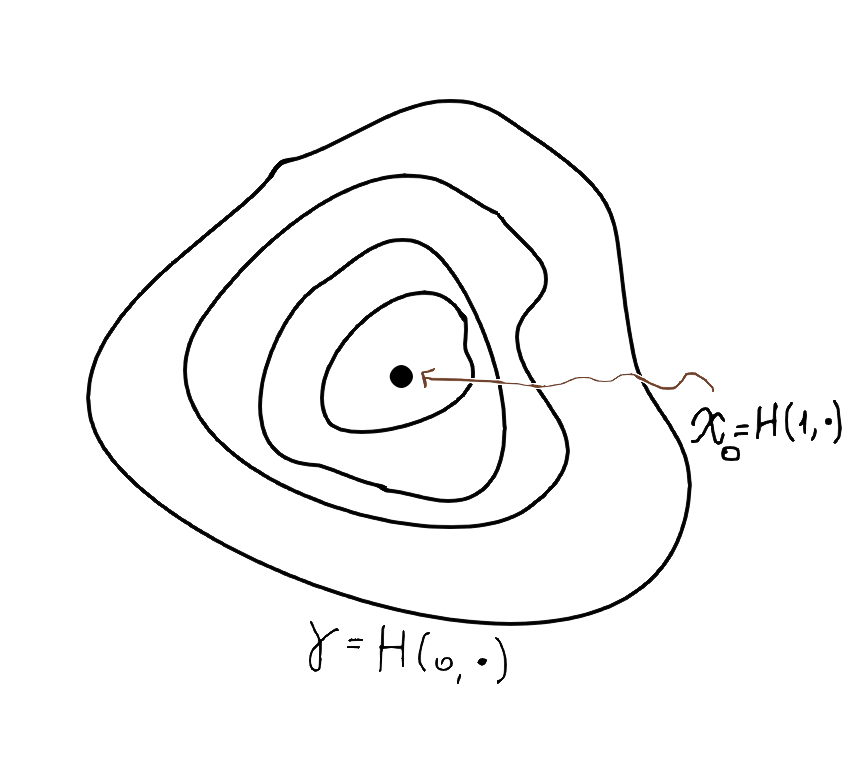
\includegraphics{immagini/omotopia.png}
	\caption{Rappresentazione di un'omotopia: la curva $\gamma$ viene strizzata fino a diventare il punto $x_0$.}
\end{figure}
\begin{definition}[insieme semplicemente connesso]
	Diremo che $E \subseteq \mathbb{R}^n$ è un insieme semplicemente connesso se
	\begin{enumerate}[label=\protect\circled{\arabic*}]
		\item è connesso per archi;
		\item $\forall \gamma \in C^0([a, b], E)$ chiusa ha un punto $x_0 \in E$ a cui è omotopa in $E$.
	\end{enumerate}
\end{definition}
\begin{remark}
	Un esempio di insieme semplicemente connesso è $\Omega = \mathbb{R}^2 \setminus \{(x, y) \in \mathbb{R}^2 : y = 0, x > 0 \}$: questo perché è possibile deformare con continuità la curva chiusa $\gamma$ affinché scavalchi la parte dell'insieme esclusa. Un insieme non semplicemente connesso è $\mathbb{R}^2 \setminus \{ (0, 0) \}$ 
	siccome prendendo una curva sufficientemente vicina all'origine, per esempio, e un raggio sufficientemente grande la curva sarebbe costretta a passare per l'origine che è però esclusa.
	Per $n > 2$ avremo che $\mathbb{R}^n \setminus \{ (0, 0) \}$ è semplicemente connesso siccome è possibile deformare la curva, sfruttando le dimensioni "in più" rispetto ad $\mathbb{R}^2$, per scavalcare l'origine.
\end{remark}
\begin{remark}
	Sia $\Omega = \mathbb{R} \setminus S$ e $S = q + \mathbb{R}v$. $S=\{q+tv : t \in \mathbb{R} \}, q, v \in \mathbb{R}^3$, ovvero lo spazio tridimensionale senza una realtà. Allora $\Omega$ non è semplicemente connesso, siccome prendendo una circonferenza sufficientemente vicina alla retta e con un raggio maggiore della distanza dal punto alla retta, la curva sarebbe costretta a "toccare" la retta per poter essere omotopa ad un punto, pertanto
	non è un insieme semplicemente connesso.
\end{remark}
\begin{prop}[gli insiemi convessi sono semplicemente connessi]
	Sia $E \subseteq \mathbb{R}^n$, allora $E$ è semplicemente connesso
\end{prop}
\begin{proof}
	Se $E$ è convesso e $\gamma: [a, b] \to E$ è chiusa e continua scelgo $x_0 \in E$ e osservo che, preso
	\begin{align*}
	&H(s,t) = sx_0 + \gamma(t) (1 - s) & &0 \leq s \leq 1,
	\end{align*}
	per la convessità di $E$ avremo che $H(s, t) \in E$. Avremo per $s = 0$ che $H(0, t)=\gamma(t)$ e per $s=1$ che $H(1, t)=x_0$. Siccome $H$ è continua, avremo che $H$ è un'omotopia in $E$ tra $\gamma$ e $x_0$.
\end{proof}
\begin{theorem}
	Sia $\Omega \subseteq \mathbb{R}^n$ aperto e semplicemente connesso e sia $\omega \in C^1(\Omega, (\mathbb{R}^n)^*)$. Allora
	\begin{align*}
		\omega \text{ è chiusa } \iff \omega \text{ è esatta }. 
	\end{align*}
	Equivalentemente, se $F \in C^1(\Omega, \mathbb{R}^n)$ allora
	\begin{align*}
		F \text{ è irrotazionale } \iff F \text{ è conservativo }.
	\end{align*}
\end{theorem}
\begin{proof} la dimostrazione verrà fatta, senza perdere di generalità, nel caso delle $1-$forme differenziali. \\
	$\boxed{\Leftarrow}:$ già dimostrato nella proposizione~\ref{prop:esattezza_imp_chiusura} \\
	$\boxed{\Rightarrow}:$ %questa dimostrazione si rifà a delle proprietà del \emph{prodotto wedge}, che trovate nelle appendici.
	%Sappiamo che $\omega = a_1(x)dx_1 + \ldots + a_n(x)dx_n$ e, siccome la forma $\omega$ è chiusa, abbiamo che $d\omega = 0$, dunque
	%$$
	%d\omega = d(a_1(x)dx_1 + \ldots a_n(x)dx_n) = \sum_{i=1}^n da_i \wedge dx_i = \sum_{i=1}^n \left( \sum_{j=1}^n \frac{\partial a_i}{\partial x_j} dx_j \right) \wedge dx_i \stackrel{\text{linearità del prodotto wedge}}{=} \sum_{i=1}^n \sum_{j=1}^n \frac{\partial a_i}{\partial x_j} dx_j \wedge dx_i
	%$$
	fissiamo $x_0 \in \Omega$ e, preso $x \in \Omega$, consideriamo la funzione
	$$
		F(x) = \int_\gamma \omega
	$$
	dove $\gamma(t) : [0, 1] \mapsto \Omega$ è una curva con $\gamma(t)=(1-t) x_0 + tx$. Per definizione di integrale curvilineo di seconda specie avremo che
	$$
		\int_0^1 \omega(\gamma(t)) \dot{\gamma}(t) dt = \int_0^1 \omega((1-t)x_0 + tx)(x-x_0)dt
	$$
	ma possiamo derivare sotto il segno di integrale (la derivata di $\omega \circ \gamma$ esiste ed è continua siccome composizione di funzioni derivabili lungo una direzione $x_j$):
	\begin{align*}
	&\partial_{x_j} F(x) = \int_0^1 \partial_{x_j} \left(\sum_{i=1}^n a_i((1-t)x_0 + tx)(x_i-x_{0_i}) \right) = \int_0^1 \left(a_j((1-t)x_0 + tx) + \right. \\
	&+\sum_{i=1}^n t\frac{\partial a_i}{\partial x_j}((1-t)x_0 + tx)(x_i - x_{0_i}) \Bigg) dt
	\end{align*}
	adesso osserviamo che la chiusura della $1-$forma differenziale implica che $\forall 1 \leq i < j \leq n$
	$$
	\frac{\partial a_i}{\partial x_j} = \frac{\partial a_j}{\partial x_i}.
	$$
	Inoltre osserviamo che, tramite il teorema del differenziale della composizione, abbiamo che 
	$$
		\frac{\partial}{\partial t} a_j((1-t)x_0 + tx) = Da_j((1-t)x_0 + tx) \, D((1-t)x_0 + tx)(t) = \sum_{i=1}^n \frac{\partial a_j}{\partial x_i}(x_i - x_{0_i})
	$$
	dunque, effettuando questa sostituzione nell'integrale di sopra, otterremo che
	\begin{align*}
	&\partial_{x_j} F(x) = \int_0^1 \partial_{x_j} \left(a_j((1-t)x_0 + tx) + \sum_{i=1}^n t\frac{\partial a_j}{\partial x_i} \left( ((1-t)x_0 + tx) (x_i - x_{0_i}) \right) \right) dt = \\
	&=\int_0^1 \left( a_j((1-t)x_0 + tx) + t\frac{\partial}{\partial t} \left[ a_j((1-t)x_0 + tx) \right] \right)dt = \int_0^1 \frac{\partial}{\partial t} \left( ta_j((1-t)x_0 + tx) \right)dt = \\
	&=a_j(x) 
	\end{align*}
	dunque $dF=\omega$, il che conclude la dimostrazione.
\end{proof}
\subsection{Campi vettoriali radiali}
\begin{definition}[campo vettoriale radiale]
	Consideriamo $h: (0, +\infty) \mapsto \mathbb{R}$ continua e $F: \mathbb{R}^n \setminus \{\underline{0} \} \to \mathbb{R}^n$ con $F(x) = h(|x|)x$.
	Diremo allora che $F$ è un campo vettoriale radiale.
\end{definition}
\begin{remark}
Siccome $\nabla |x| = \frac{x}{|x|} \, \forall x \neq \underline{0}$ allora $F(x) = |x|h(|x|)\frac{x}{|x|} \implies F(x) = |x| \, h(|x|)\nabla |x|$
\end{remark}
\begin{prop}[i campi radiali sono conservativi]
	Sia $F$ un campo vettoriale radiale, allora $F$ è conservativo
\end{prop}
\begin{proof}
	Possiamo pensare di definire
	$$
	U(s) = \int_1^s t h(t)dt \text{ con } s > 0 
	$$
	e posto $V(x) = U(|x|) \implies$
	$$
	\implies \nabla V(x) = \sum_{j=1}^n \frac{\partial}{\partial x_j} U(|x|)e_j
	$$
	ma osserviamo che $\frac{\partial U(|x|)}{\partial x_j} = \frac{\partial U(|x|)}{\partial |x|} \frac{\partial |x|}{\partial x_j} = U'(|x|) \frac{x_j}{|x|}$ dove osserviamo che $\frac{\partial |x|}{\partial x_j} = \frac{1}{\cancel{2}} \frac{\cancel{2}x_j}{\sqrt{\sum\limits_{i=1}^n x_i^2}}$
	$$
		\sum_{j=1}^n U'(|x|) \frac{x_j}{|x|}e_j = \frac{U'(|x|)}{|x|} \sum_{j=1}^n x_j e_j = \frac{U'(|x|)}{|x|} |x| = U'(|x|) = |x| \, h(|x|)
	$$
	dove si è usato il teorema fondamentale del calcolo per calcolare la derivata di $U(|x|)$ rispetto a $|x|$ siccome $\frac{\partial}{\partial |x|} = \frac{\partial}{\partial |x|} \int_1^{|x|} t h(t) dt = th(t)|_{t=|x|} = |x|h(|x|)$
\end{proof}
\begin{remark}
	Osserviamo che per $n=2$ il nostro campo vettoriale è definito su $\mathbb{R}^2 \setminus \{ (0, 0) \}$, che ricordiamo essere un insieme non semplicemente connesso. Detto questo, non è detto che non vi siano delle forme differenziali esatte: un esempio
	è il campo gravitazionale che è un campo conservativo.
\end{remark}
Similmente, possiamo definire le $1-$forme differenziali radiali nella seguente maniera
\begin{definition}[$1-$forma differenziale radiale]
	Sia $h(x) \in C^0((0, +\infty), \mathbb{R})$ e sia $\omega \in C^{\infty}(\mathbb{R}^n \setminus \{ \underline{0} \}, (\mathbb{R}^n)^*)$ è una $1-$ forma differenziale radiali se
	$$
		\omega(x) = h(|x|)\sum_{j=1}^n x_j dx_j
	$$
\end{definition}
Come prima, avremo che è esatta con primitiva $P(x)=U(|x|)$, dove $U(s) = \int_1^s th(t)dt$ e $dP(x)=\omega(x)$.